\documentclass[10pt]{article}
\usepackage[margin=0.78in]{geometry}
\usepackage[T1]{fontenc}
\usepackage{lmodern}
\usepackage{microtype}
\usepackage{booktabs}
\usepackage{array}
\usepackage{xcolor}
\usepackage{hyperref}
\usepackage{fancyhdr}
\usepackage{caption}
\usepackage{enumitem}
\usepackage{siunitx}
\usepackage{seqsplit}
\usepackage{tikz}
\usepackage{pgfplots}
\usepgfplotslibrary{groupplots}
\usetikzlibrary{arrows.meta,positioning,shapes.geometric}
\pgfplotsset{compat=1.18}

\definecolor{vblue}{HTML}{1F5A94}
\definecolor{vcyan}{HTML}{58A7B8}
\definecolor{vgold}{HTML}{D89531}
\definecolor{vgreen}{HTML}{3B8B5A}
\definecolor{vred}{HTML}{B7473C}
\definecolor{vgray}{HTML}{69727D}
\hypersetup{
  colorlinks=true,
  linkcolor=vblue,
  urlcolor=vblue,
  citecolor=vblue,
  pdftitle={Production Full-CMG Benchmarks for VCkss},
  pdfauthor={VCkss development report},
  pdfsubject={Private 0.4.0-alpha.1 benchmark and qualification evidence}
}
\setlist{nosep,leftmargin=*}
\captionsetup{font=small,labelfont=bf}
\pagestyle{fancy}
\fancyhf{}
\lhead{VCkss full-CMG alpha benchmark}
\rhead{\thepage}
\setlength{\headheight}{13.6pt}
% Exact source-bound alpha qualification and benchmark data.
\newcommand{\PackageVersion}{0.4.0-alpha.1}
\newcommand{\ReportDate}{27 August 2026}
\newcommand{\RuntimeCommit}{4b6874ededa1244bca389e4ee82148b42b9693a1}
\newcommand{\RuntimeShort}{4b6874e}
\newcommand{\MacQualificationCommit}{4dafec6734af4b8d3c25785f268f19f69f780684}
\newcommand{\LinuxQualificationCommit}{992eba0947ca155c534f532750fc202e41ecf978}
\newcommand{\CmgCommit}{dbefbc5e3b442c6dde6e7861a66d82fd5ed24f10}
\newcommand{\CmgShort}{dbefbc5}
\newcommand{\SupplyShort}{4dafec6}
\newcommand{\MacInputSha}{19744b8418ffff82461527d7426cdc976dce18bf36597555d19bf847dec5afbe}
\newcommand{\SccInputSha}{1748ca2a6a46f248e05c0329407e7e7708ec7628c1ffce5f0e06ee264bdf0575}
\newcommand{\MacRows}{1,966,080}
\newcommand{\MacWorkers}{327,680}
\newcommand{\SccRows}{8,201,888}
\newcommand{\SccWorkers}{117,529}
\newcommand{\TimeAxisMax}{120}
\newcommand{\RssAxisMax}{14}
\newcommand{\MacVckss}{74.774}
\newcommand{\MacMatlab}{104.489}
\newcommand{\MacRatio}{0.716}
\newcommand{\MacSpeedup}{1.397}
\newcommand{\MacPrivate}{81.145}
\newcommand{\MacPrivateRatio}{0.921}
\newcommand{\SccVckss}{19.097}
\newcommand{\SccMatlab}{33.058}
\newcommand{\SccRatio}{0.578}
\newcommand{\SccSpeedup}{1.731}
\newcommand{\SccPrivate}{33.942}
\newcommand{\SccPrivateRatio}{0.563}
\newcommand{\SccTwoXText}{remains above the 0.5 threshold}
\newcommand{\MacRss}{5.121}
\newcommand{\MacMatlabRss}{12.161}
\newcommand{\MacRssRatio}{0.421}
\newcommand{\SccRss}{2.788}
\newcommand{\SccMatlabRss}{11.417}
\newcommand{\SccRssRatio}{0.244}
\newcommand{\MacFront}{2.933}
\newcommand{\MacSetupRhs}{2.411}
\newcommand{\MacSolve}{59.826}
\newcommand{\MacExtract}{4.523}
\newcommand{\MacOtherNative}{5.081}
\newcommand{\SccFront}{9.298}
\newcommand{\SccSetupRhs}{0.914}
\newcommand{\SccSolve}{4.131}
\newcommand{\SccExtract}{1.755}
\newcommand{\SccOtherNative}{3.000}
\newcommand{\MacIngest}{0.032}
\newcommand{\MacCanonical}{0.573}
\newcommand{\MacGraph}{0.447}
\newcommand{\MacCompression}{0.522}
\newcommand{\MacPlan}{0.152}
\newcommand{\MacNativeSolve}{71.841}
\newcommand{\MacCmgGraph}{0.428}
\newcommand{\MacHierarchy}{0.133}
\newcommand{\MacRhs}{1.850}
\newcommand{\SccIngest}{0.245}
\newcommand{\SccCanonical}{1.719}
\newcommand{\SccGraph}{0.546}
\newcommand{\SccCompression}{1.397}
\newcommand{\SccPlan}{1.019}
\newcommand{\SccNativeSolve}{9.799}
\newcommand{\SccCmgGraph}{0.055}
\newcommand{\SccHierarchy}{0.015}
\newcommand{\SccRhs}{0.844}
\newcommand{\MacIterations}{4,817}
\newcommand{\MacOperatorApps}{5,418}
\newcommand{\MacCmgApps}{4,817}
\newcommand{\MacRefineAttempts}{0}
\newcommand{\MacRefinedCols}{0}
\newcommand{\MacReducedResidual}{$7.862\times10^{-6}$}
\newcommand{\MacCompleteResidual}{$6.971\times10^{-6}$}
\newcommand{\SccIterations}{7,001}
\newcommand{\SccOperatorApps}{8,886}
\newcommand{\SccCmgApps}{7,001}
\newcommand{\SccRefineAttempts}{35}
\newcommand{\SccRefinedCols}{1,284}
\newcommand{\SccReducedResidual}{$1.541\times10^{-3}$}
\newcommand{\SccCompleteResidual}{$9.975\times10^{-6}$}
\newcommand{\MacMatDiffWorker}{$6.19\times10^{-6}$}
\newcommand{\MacMatDiffFirm}{$1.44\times10^{-5}$}
\newcommand{\MacMatDiffCov}{$1.11\times10^{-5}$}
\newcommand{\MacMatDiffTotal}{$1.64\times10^{-6}$}
\newcommand{\MacPrivDiffWorker}{0}
\newcommand{\MacPrivDiffFirm}{0}
\newcommand{\MacPrivDiffCov}{0}
\newcommand{\MacPrivDiffTotal}{0}
\newcommand{\SccMatDiffWorker}{$1.48\times10^{-3}$}
\newcommand{\SccMatDiffFirm}{$7.63\times10^{-5}$}
\newcommand{\SccMatDiffCov}{$1.07\times10^{-4}$}
\newcommand{\SccMatDiffTotal}{$1.62\times10^{-3}$}
\newcommand{\SccPrivDiffWorker}{$2.20\times10^{-9}$}
\newcommand{\SccPrivDiffFirm}{$3.67\times10^{-9}$}
\newcommand{\SccPrivDiffCov}{$2.45\times10^{-9}$}
\newcommand{\SccPrivDiffTotal}{$9.75\times10^{-10}$}
\newcommand{\MacForecast}{32.828}
\newcommand{\MacAdmitted}{19.500}
\newcommand{\MacRetained}{1.184}
\newcommand{\SccForecast}{9.788}
\newcommand{\SccAdmitted}{7.133}
\newcommand{\SccRetained}{0.095}
\newcommand{\SccQualifierJob}{7330577}
\newcommand{\SccQualifierStatus}{\code{failed=0} and \code{exit\_status=0}}


\newcommand{\code}[1]{\texttt{#1}}
\newcommand{\pass}{\textcolor{vgreen}{\textbf{PASS}}}
\newcommand{\deferred}{\textcolor{vgold}{\textbf{DEFERRED}}}

\title{Production Full-CMG Benchmarks for VCkss\\
\large Private \PackageVersion{} candidate versus maintained MATLAB KSS}
\author{VCkss development report}
\date{\ReportDate}

\begin{document}
\maketitle

\begin{abstract}
This report qualifies the ordinary-build \code{CMG\_FULL\_V2} route in VCkss
against the maintained MATLAB KSS implementation on two registered hard
problems. Both use 200 randomized projections and four application workers,
with one cold and five position-balanced warm runs. At source
\texttt{\RuntimeShort{}}, VCkss's median complete-command time is
\MacRatio{} times MATLAB on the macOS 8,192-firm case and \SccRatio{} times
MATLAB on fixed CZ18. Peak process-tree memory is \MacRssRatio{} and
\SccRssRatio{} times MATLAB, respectively. Both cases pass the selected alpha
gate---faster than matched MATLAB, no more than five percent slower than the
source-bound private winner, and all statistical, complete-residual, memory,
state, and lifecycle checks passing. The aspirational 2x MATLAB target is not
claimed.
\end{abstract}

\section{Decision and scope}

The promoted implementation directly solves VCkss's prepared hybrid
worker--firm Laplacian. It vendors exact standalone CMG source
\texttt{\CmgShort{}} and reuses one graph, hierarchy, Rayon pool, parallel
plan, and admitted workspace pool across 601 fit, leverage, and target right-
hand sides. It does not route exact results through JLA, does not use the
retired simplified hierarchy, and does not select a fallback after estimator
RNG begins.

The production cell is deliberately narrow: no controls, weights, target
weights, or explicit deletion ID; match deletion, joint nuisance, mover
headline, JLA, automatic engine/preconditioner/batch, Counter-V1, and an
effective observation key. It is available through explicit
\code{backend(rust)} and, on qualified macOS/Linux runtimes, eligible
\code{backend(auto)} requests. Explicit \code{backend(mata)} remains
permanent. Windows, a public tag, and public distribution are outside this
report.

\begin{figure}[h]
\centering
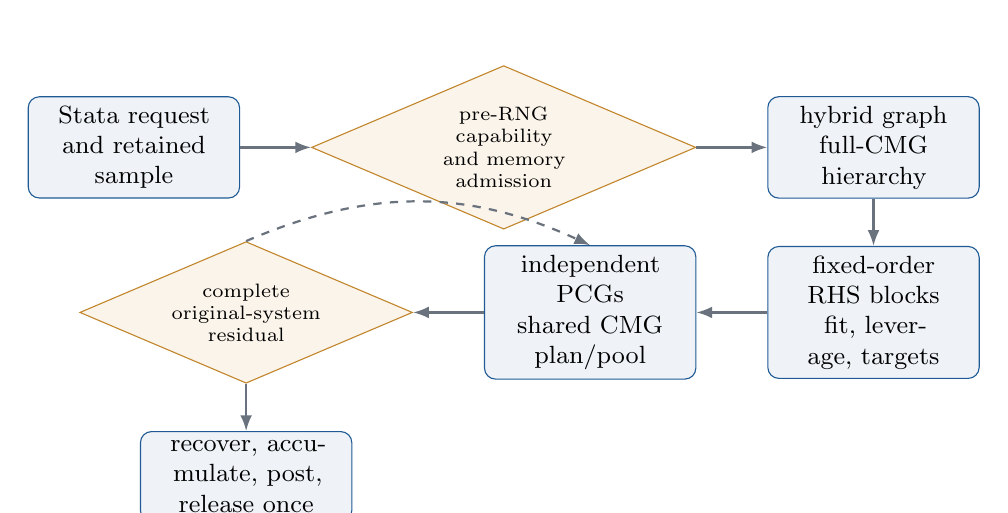
\begin{tikzpicture}[
  node distance=6mm and 9mm,
  box/.style={draw=vblue,rounded corners,fill=vblue!7,align=center,
    minimum height=9mm,text width=2.45cm,font=\small},
  gate/.style={draw=vgold!90!black,diamond,aspect=2.35,fill=vgold!10,
    align=center,font=\scriptsize,text width=2.15cm,inner sep=1.5pt},
  arrow/.style={-{Latex[length=2mm]},thick,vgray}]
\node[box] (stata) {Stata request\\and retained sample};
\node[gate,right=of stata] (admit) {pre-RNG capability and memory admission};
\node[box,right=of admit] (graph) {hybrid graph\\full-CMG hierarchy};
\node[box,below=of graph] (rhs) {fixed-order RHS blocks\\fit, leverage, targets};
\node[box,left=of rhs] (solve) {independent PCGs\\shared CMG plan/pool};
\node[gate,left=of solve] (cert) {complete original-system residual};
\node[box,below=of cert] (post) {recover, accumulate, post, release once};
\draw[arrow] (stata) -- (admit);
\draw[arrow] (admit) -- (graph);
\draw[arrow] (graph) -- (rhs);
\draw[arrow] (rhs) -- (solve);
\draw[arrow] (solve) -- (cert);
\draw[arrow] (cert) -- (post);
\draw[arrow,dashed] (cert.north) to[bend left=24] (solve.north);
\end{tikzpicture}
\caption{Production dataflow. Admission and the deterministic refinement
schedule are frozen before Counter-V1. A failed selected route returns a typed
error; it never changes estimator or backend after RNG.}
\end{figure}

\section{Registered protocol}

\begin{tabular}{>{\raggedright\arraybackslash}p{0.22\linewidth}p{0.71\linewidth}}
\toprule
Item & Registered value \\
\midrule
Production source & \texttt{\footnotesize\expandafter\seqsplit\expandafter{\RuntimeCommit}} \\
CMG source & \texttt{\footnotesize\expandafter\seqsplit\expandafter{\CmgCommit}} \\
Toolchain & Rust 1.85.1; VCkss MSRV 1.85; VCkss edition 2021; vendored CMG edition 2024 \\
Estimator & JLA, 200 probes, four workers, one cold plus five alternating warm runs \\
Tolerances & fit $10^{-10}$; randomized probes $10^{-6}$; fit inner start $10^{-12}$ \\
Residual gate & complete original system $\leq\max(10^{-11},10\tau)$; same-route 10x refinement only \\
macOS & \MacRows{} rows, \MacWorkers{} workers, 8,192 firms; Stata/MP 19; MATLAB R2024b Update 5 \\
SCC & \SccRows{} rows, \SccWorkers{} workers, 10,603 firms; Stata/MP 19; MATLAB R2024b Update 3 \\
Timing & complete estimator command; medians of five warm repetitions; launch order position-balanced \\
Memory & complete process-tree peak RSS; VCkss also receipts pre-RNG forecast, admitted peak, and retained bytes \\
\bottomrule
\end{tabular}

The two inputs are fixed by SHA-256: macOS
\texttt{\footnotesize\MacInputSha} and SCC
\texttt{\footnotesize\SccInputSha}. MATLAB source and runtime trees are
separately hashed. Queue wait, source deployment, compilation, MATLAB pool
startup, and MEX setup are reported but excluded from the complete estimator
command in both applications.

\section{End-to-end performance}

\begin{figure}[h]
\centering
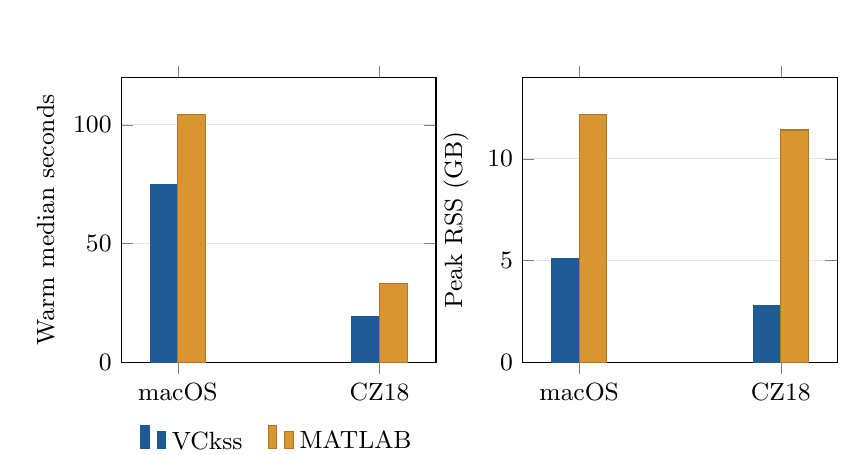
\begin{tikzpicture}
\begin{groupplot}[
  group style={group size=2 by 1,horizontal sep=1.1cm},
  ybar=0pt,width=0.46\textwidth,height=5.2cm,
  symbolic x coords={macOS,CZ18},xtick=data,
  enlarge x limits=0.28,ymajorgrids=true,grid style={gray!20},
  legend style={draw=none,font=\small,at={(0.5,-0.20)},anchor=north,legend columns=2,
    /tikz/every even column/.append style={column sep=0.25cm}},
  tick label style={font=\small},label style={font=\small}]
\nextgroupplot[ylabel={Warm median seconds},ymin=0,ymax=\TimeAxisMax]
\addplot[fill=vblue,draw=vblue] coordinates {(macOS,\MacVckss) (CZ18,\SccVckss)};
\addplot[fill=vgold,draw=vgold!80!black] coordinates {(macOS,\MacMatlab) (CZ18,\SccMatlab)};
\legend{VCkss,MATLAB}
\nextgroupplot[ylabel={Peak RSS (GB)},ymin=0,ymax=\RssAxisMax]
\addplot[fill=vblue,draw=vblue] coordinates {(macOS,\MacRss) (CZ18,\SccRss)};
\addplot[fill=vgold,draw=vgold!80!black] coordinates {(macOS,\MacMatlabRss) (CZ18,\SccMatlabRss)};
\end{groupplot}
\end{tikzpicture}
\caption{Median complete-command time and process-tree peak RSS at four
application workers. Lower is better.}
\end{figure}

\begin{table}[h]
\centering
\caption{Warm-median promotion results.}
\begin{tabular}{lrrrrrr}
\toprule
Case & VCkss (s) & MATLAB (s) & Ratio & Speed advantage & Private (s) & Prod./private \\
\midrule
macOS 8,192-firm & \MacVckss & \MacMatlab & \MacRatio & \MacSpeedup{}x & \MacPrivate & \MacPrivateRatio \\
SCC fixed CZ18 & \SccVckss & \SccMatlab & \SccRatio & \SccSpeedup{}x & \SccPrivate & \SccPrivateRatio \\
\bottomrule
\end{tabular}
\end{table}

Both selected promotion rules pass. Neither case regresses from its private
winner; production is faster in both. The macOS ratio is above the 0.5 stretch
target, and the SCC result \SccTwoXText. No 2x release claim is made.

\section{Where command time goes}

\begin{figure}[h]
\centering
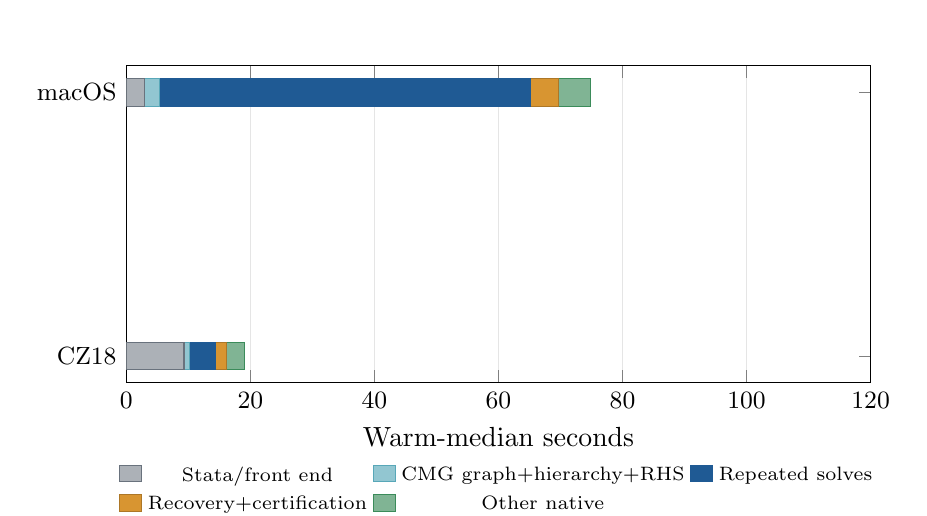
\begin{tikzpicture}
\begin{axis}[
  xbar stacked,width=0.91\textwidth,height=5.6cm,
  symbolic y coords={CZ18,macOS},ytick=data,
  xlabel={Warm-median seconds},xmin=0,xmax=\TimeAxisMax,
  xmajorgrids=true,grid style={gray!20},
  legend style={draw=none,font=\scriptsize,at={(0.5,-0.23)},anchor=north,legend columns=3},
  tick label style={font=\small}]
\addplot[fill=vgray!55,draw=vgray] coordinates {(\MacFront,macOS) (\SccFront,CZ18)};
\addplot[fill=vcyan!65,draw=vcyan] coordinates {(\MacSetupRhs,macOS) (\SccSetupRhs,CZ18)};
\addplot[fill=vblue,draw=vblue] coordinates {(\MacSolve,macOS) (\SccSolve,CZ18)};
\addplot[fill=vgold,draw=vgold!80!black] coordinates {(\MacExtract,macOS) (\SccExtract,CZ18)};
\addplot[fill=vgreen!65,draw=vgreen] coordinates {(\MacOtherNative,macOS) (\SccOtherNative,CZ18)};
\legend{Stata/front end,CMG graph+hierarchy+RHS,Repeated solves,Recovery+certification,Other native}
\end{axis}
\end{tikzpicture}
\caption{A reconciled decomposition of complete-command medians. Categories
sum to the reported command median; ``other native'' is the receipted native
solve remainder after the separately timed full-CMG phases.}
\end{figure}

\begin{table}[h]
\centering
\caption{Detailed median native and full-CMG receipts (seconds).}
\begin{tabular}{lrr@{\qquad}lrr}
\toprule
Phase & macOS & CZ18 & Phase & macOS & CZ18 \\
\midrule
Native ingest & \MacIngest & \SccIngest & Full-CMG graph & \MacCmgGraph & \SccCmgGraph \\
Canonicalization & \MacCanonical & \SccCanonical & Hierarchy/plan & \MacHierarchy & \SccHierarchy \\
Native graph & \MacGraph & \SccGraph & RHS construction & \MacRhs & \SccRhs \\
Compression & \MacCompression & \SccCompression & Repeated solve & \MacSolve & \SccSolve \\
Native plan & \MacPlan & \SccPlan & Extract/recover/certify & \MacExtract & \SccExtract \\
Native solve total & \MacNativeSolve & \SccNativeSolve & Complete command & \MacVckss & \SccVckss \\
\bottomrule
\end{tabular}
\end{table}

Repeated independent solves are still the largest macOS phase. On CZ18,
Stata/native preparation and data movement are comparably important after the
faster, smaller Laplacian solve. The shortest next optimization path is
therefore platform/case specific: improve repeated full-CMG applications on
the synthetic headline while profiling front-end preparation on CZ18. Retired
fused, mixed-precision, and pass-fused prototypes remain disabled because they
did not beat the scalar winner under the registered end-to-end rule.

\section{Solver work, residuals, and statistical outputs}

\begin{table}[h]
\centering
\caption{Warm-median full-CMG work and numerical certification.}
\begin{tabular}{lrr}
\toprule
Measure & macOS & SCC CZ18 \\
\midrule
Right-hand sides & 601 & 601 \\
PCG iterations & \MacIterations & \SccIterations \\
Operator applications & \MacOperatorApps & \SccOperatorApps \\
CMG applications & \MacCmgApps & \SccCmgApps \\
Refinement attempts / columns & \MacRefineAttempts{} / \MacRefinedCols & \SccRefineAttempts{} / \SccRefinedCols \\
Maximum reduced residual & \MacReducedResidual & \SccReducedResidual \\
Maximum complete residual & \MacCompleteResidual & \SccCompleteResidual \\
Default probe limit & $10^{-5}$ & $10^{-5}$ \\
\bottomrule
\end{tabular}
\end{table}

CZ18's attempt-level reduced maximum may exceed the final threshold because
the receipt retains the first attempt. The frozen schedule deterministically
re-solves only failing columns at a 10x tighter inner tolerance. Every selected
column passes the independent complete original worker-plus-firm system before
posting. Refinement never changes RNG draws, hierarchy, result family, or
backend.

\begin{table}[h]
\centering
\caption{Corrected-target comparison. MATLAB differences are descriptive;
private-winner differences use common Counter-V1 probes and are release-blocking.}
\begin{tabular}{lrrrr}
\toprule
& \multicolumn{2}{c}{Absolute VCkss--MATLAB difference}
& \multicolumn{2}{c}{Absolute production--private difference} \\
Target & macOS & CZ18 & macOS & CZ18 \\
\midrule
Worker variance & \MacMatDiffWorker & \SccMatDiffWorker & \MacPrivDiffWorker & \SccPrivDiffWorker \\
Firm variance & \MacMatDiffFirm & \SccMatDiffFirm & \MacPrivDiffFirm & \SccPrivDiffFirm \\
Covariance & \MacMatDiffCov & \SccMatDiffCov & \MacPrivDiffCov & \SccPrivDiffCov \\
Total & \MacMatDiffTotal & \SccMatDiffTotal & \MacPrivDiffTotal & \SccPrivDiffTotal \\
\bottomrule
\end{tabular}
\end{table}

MATLAB uses a different RNG, solver contract, and, on CZ18, target-weight
convention. It does not emit a compatible numerical MCSE. Its point
differences therefore document statistical agreement but are not falsely
presented as pathwise equality. The common-probe private comparisons all pass
the registered scale/MCSE-aware rule. Data, caller RNG, sort RNG,
\code{e(sample)}, accounting, target identity, typed status, and idle-registry
checks pass in every accepted run.

\section{Memory, cancellation, and lifecycle}

\begin{table}[h]
\centering
\caption{Warm-median and receipted memory (GB, decimal).}
\begin{tabular}{lrr}
\toprule
Measure & macOS & SCC CZ18 \\
\midrule
Pre-RNG conservative forecast & \MacForecast & \SccForecast \\
Admitted full-CMG peak & \MacAdmitted & \SccAdmitted \\
Actual retained native storage & \MacRetained & \SccRetained \\
Observed VCkss process-tree RSS & \MacRss & \SccRss \\
Observed MATLAB process-tree RSS & \MacMatlabRss & \SccMatlabRss \\
\bottomrule
\end{tabular}
\end{table}

The forecast covers retained input, canonicalization, raw match preparation,
hybrid and CMG graph copies, hierarchy bounds, parallel plan, thread/workspace
pool, RHS/results, extraction, residual checks, ABI copies, transients, and an
allocator allowance. Graph and hierarchy construction completes before
Counter-V1, actual retained sizes are reconciled to the forecast, and a failed
admission returns without estimator RNG.

Owned work runs under a coordinator worker. The Stata caller thread polls
UserBreak and sets an atomic cancellation token observed by preparation, CMG,
PCG, recovery, and certification code; Rayon workers never call the Stata API.
Success, memory rejection, cancellation, convergence failure, corrupt receipt,
posting failure, panic, and stale-handle tests require one terminal generation,
exactly-once release, and an idle registry.

\section{Platform qualification and provenance}

The same runtime source, packaged at macOS receipt tip
\texttt{\footnotesize\expandafter\seqsplit\expandafter{\MacQualificationCommit}},
passed macOS arm64 and x86-64 thin plugins, the universal plugin, Rosetta
execution, clean installation, Rust/C/ABI checks, full-CMG explicit and
automatic routing, cancellation, memory/refinement, and lifecycle coverage.
SCC job \SccQualifierJob{} used Linux qualifier source
\texttt{\footnotesize\expandafter\seqsplit\expandafter{\LinuxQualificationCommit}},
built a normal Linux x86-64 plugin from the deterministic bundle, and ran the
locked Rust, C, ABI, Stata full-suite, and clean-install gates under Stata/MP
19. Its wrapper and \code{qacct} records report \SccQualifierStatus.

The local source-bound supply-chain gate at receipt commit
\texttt{\SupplyShort{}} audits the workspace, Stata-backend, and fuzz lockfiles
with \code{cargo-audit 0.22.2}; zero vulnerabilities and warnings are accepted.
Four deterministic CycloneDX 1.5 SBOMs record 53 components, licenses, package
URLs, and checksums. Human license/provenance approval remains required before
any public distribution.

\section{Acceptance and limitations}

\begin{tabular}{>{\raggedright\arraybackslash}p{0.52\linewidth}p{0.16\linewidth}p{0.24\linewidth}}
\toprule
Gate & Status & Evidence \\
\midrule
Faster than matched MATLAB on both registered cases & \pass & ratios \MacRatio{}, \SccRatio{} \\
No more than 5\% slower than private winner & \pass & ratios \MacPrivateRatio{}, \SccPrivateRatio{} \\
Complete original-system residuals & \pass & within $10^{-5}$ in both cases \\
Corrected-target/common-probe policy & \pass & all four targets, both cases \\
Declared memory and RSS rule & \pass & no budget breach; RSS below MATLAB \\
macOS arm64/universal/Rosetta and SCC Linux & \pass & exact-source receipts \\
Windows and public release & \deferred & no claim, binary, tag, or public release \\
2x MATLAB development target & \deferred & directional target, not alpha gate \\
\bottomrule
\end{tabular}

These are two registered hard cases, not a universal performance guarantee.
The machines differ, MATLAB retains native implementation choices, and five
warm repetitions support engineering medians rather than formal confidence
intervals. The report does not claim econometric standard errors: VCkss posts
point estimates and numerical Monte Carlo error only, with no \code{e(V)}.

\section{Reproduction commands}

All commands were run from a clean \code{main} checkout. The exact paths in
the receipts are retained; portable forms are:

\begin{verbatim}
rust/stata_backend/qualify_macos.sh \
  --receipt /private/tmp/vckss-alpha-4dafec6-macos-receipt.txt \
  --artifacts-dir /private/tmp/vckss-alpha-4dafec6-macos-artifacts

/opt/anaconda3/bin/python3 vckss/benchmarks/full_cmg_production/run_local.py \
  --output-dir /private/tmp/vckss-full-cmg-alpha-4b6874e \
  --input-csv /private/tmp/vckss-local-matrix-787327f/run/input/input.csv \
  --matlab-root /Users/johannes/Git/varcomp_hdfe/Monte_Carlo/LeaveOutTwoWay

rust/stata_backend/scc/deploy_linux_bundle.sh REPO RUN_ID
ssh scc RUN_DIR/source/rust/stata_backend/scc/submit_linux_qualifier.sh RUN_DIR

vckss/benchmarks/full_cmg_production/submit_scc_cz18.sh \
  20260827T023000Z-alpha-cz18-4b6874e
\end{verbatim}

Compact exact-source receipts, validator output, source and input hashes,
platform identities, wrapper records, and scheduler accounting live under
\path{vckss/benchmarks/full_cmg_production/evidence/} and
\path{rust/qualification/evidence/}. Raw SCC runs remain under
\path{/projectnb/welfgr/vckss/runs/}; disposable build/log caches are excluded
from the maintained source tree. The final protected cleanup removed 26,310
regenerable files (4.187 GB) without touching any tracked receipt or report.

\end{document}
